\documentclass[11pt]{article}
\usepackage{preamble}
\titleformat*{\section}{\Large\bfseries}
\usepackage{mathtools}
\DeclarePairedDelimiter\ceil{\lceil}{\rceil}
\DeclarePairedDelimiter\floor{\lfloor}{\rfloor}
\def\columnseprulecolor{\color{blue}}

\title{CISC 3220 Homework Chapter 6}
\author{Rachel Friedman}
\date{April 19, 2020}

\begin{document}
\maketitle

\section*{Exercises 6.1}\nointerlineskip
\noindent \rule{\linewidth}{0.01pt}\\

\subsubsection*{Question 6.1-1}\nointerlineskip
What are the minimum and maximum numbers of elements in a heap of height $h$?\\[6pt]
 \indent A heap is a balanced binary tree where all levels except the last one is completely full. Therefore, the minimum amount of elements is: $2^h$ and the maximum amount is: $2^{h+1}-1$.\\

\subsubsection*{Question 6.1-2}\nointerlineskip
Show that an $n$ element heap has height $\floor{\text{lg } n}$. \\[6pt]
\indent From the solution above, we know that the minimum amount of elements in a tree is $2^h$ and the maximum amount of elements is $2^{h+1}-1$. Obviously, the minimum amount is less than or equal to the amount of elements which is in turn less than or equal to the maximum amount of elements. Thus:
\begin{center}
\begin{minipage}{3in}
\begin{flalign*}
2^h &\leq n \leq 2^{h+1}-1\\
h &\leq \text{log } n \leq h+1 &&\text{take log on all sides}\\
h &=\floor{\text{lg } n}  &&\text{since } h \text{ is an integer} \\
\end{flalign*}\
\end{minipage}
\end{center}

\subsubsection*{Question 6.1-6}

\indent The given array is not a max heap since the subtree with 6 as its root and 7 as its left child violates the max-heap property.\\

\newpage

\section*{Exercises 6.2}\nointerlineskip
\noindent \rule{\linewidth}{0.01pt}\\

\subsubsection*{Question 6.2-1}\nointerlineskip
Illustrate \textcolor{blue}{\textbf{MAX-HEAPIFY(A, 3)}} on the array $A = \langle 27, 17, 3, 16, 13, 10, 1, 5, 7, 12, 4, 8, 9, 0 \rangle. $\\
(Note to self: top down. Running time: \textcolor{blue}{$\mathcal{O}(\text{lg } n)$)}\\

\newcommand{\hindex}[1]{\textcolor{red}{\small${#1}$}}

\begin{center}
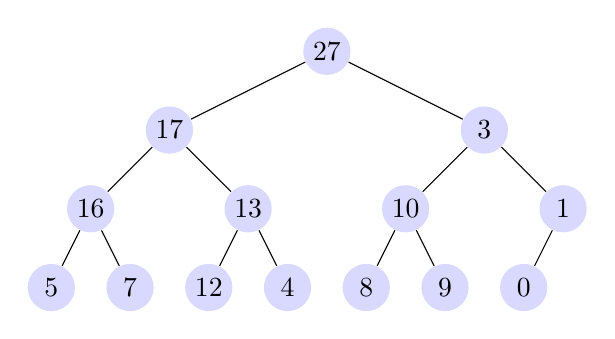
\begin{tikzpicture}
  [level distance = 10mm, node distance=0.1,
   every node/.style={fill=blue!15!white,circle, inner sep=1pt, minimum size=6mm},
   level 1/.style={sibling distance = 40mm},
   level 2/.style={sibling distance = 20mm},
   level 3/.style={sibling distance = 10mm}]
  \node {27}
     child {node{17}
       child {node {16}
          child {node {5}}
          child {node {7}}}
       child {node {13}
          child {node {12}}
          child {node {4}}}
     }
     child {node{3}
       child {node {10}
          child {node {8}}
          child {node {9}}}
       child {node {1}
          child {node {0}}
          child [missing]}
     };
\end{tikzpicture}

\vspace{30pt}

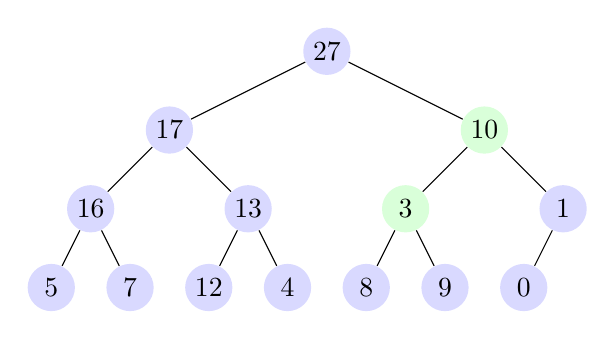
\begin{tikzpicture}
  [level distance = 10mm, node distance=0.1,
   every node/.style={fill=blue!15!white,circle, inner sep=1pt, minimum size=6mm},
   level 1/.style={sibling distance = 40mm},
   level 2/.style={sibling distance = 20mm},
   level 3/.style={sibling distance = 10mm}]
  \node {27}
     child {node{17}
       child {node {16}
          child {node {5}}
          child {node {7}}}
       child {node {13}
          child {node {12}}
          child {node {4}}}
     }
     child {node  [fill=green!15!white,circle] {10}
       child {node  [fill=green!15!white,circle] {3}
          child {node {8}}
          child {node {9}}}
       child {node {1}
          child {node {0}}
          child [missing]}
     };
\end{tikzpicture}


\vspace{30pt}

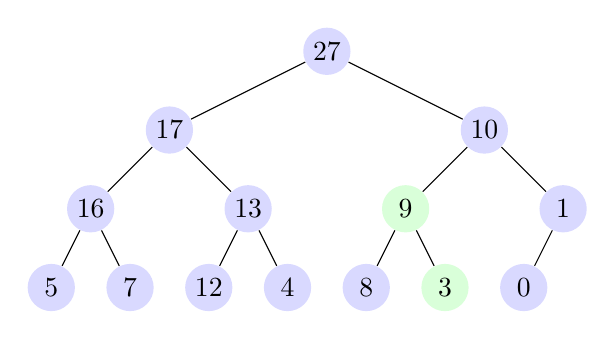
\begin{tikzpicture}
  [level distance = 10mm, node distance=0.1,
   every node/.style={fill=blue!15!white,circle, inner sep=1pt, minimum size=6mm},
   level 1/.style={sibling distance = 40mm},
   level 2/.style={sibling distance = 20mm},
   level 3/.style={sibling distance = 10mm}]
  \node {27}
     child {node{17}
       child {node {16}
          child {node {5}}
          child {node {7}}}
       child {node {13}
          child {node {12}}
          child {node {4}}}
     }
     child {node{10}
       child {node [fill=green!15!white,circle]{9}
          child {node {8}}
          child {node [fill=green!15!white,circle]{3}}}
       child {node {1}
          child {node {0}}
          child [missing]}
     };
\end{tikzpicture}
\end{center}

\vspace{30pt}

\subsubsection*{Question 6.2-3}\nointerlineskip
What is the effect of calling MAX-HEAPIFY($A, i$) when the element $A[i]$ is larger than its children?\\[12pt]
The heap is unchanged.

\newpage
\section*{Exercises 6.3}\nointerlineskip
\noindent \rule{\linewidth}{0.01pt}\\

\subsubsection*{Question 6.3-1}\nointerlineskip
Illustrate \textcolor{blue}{\textbf{BUILD-MAX-HEAP}} on the array $A=\langle 5, 3, 17, 10, 84, 19, 6, 22,9\rangle$.\\
(Note to self: bottom up. Running time is  \textcolor{blue}{$\mathcal{O}(n)$.}\\
Need more clarity as to why it's $\mathcal{O}(n)$ if the loop runs from $n/2$ to 1.)\\
\vspace{20 pt}

\begin{multicols}{2}
\begin{center}
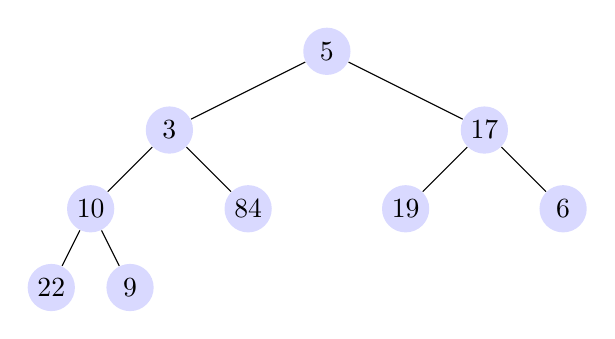
\begin{tikzpicture}
  [level distance = 10mm, node distance=0.1,
   every node/.style={fill=blue!15!white,circle, inner sep=1pt, minimum size=6mm},
   level 1/.style={sibling distance = 40mm},
   level 2/.style={sibling distance = 20mm},
   level 3/.style={sibling distance = 10mm}]
  \node {5}
     child {node{3}
       child {node {10}
          child {node {22}}
          child {node {9}}}
       child {node {84}
          child  [missing]
          child [missing]}
     }
     child {node {17}
       child {node {19}
          child  [missing]
          child [missing]}
       child {node {6}
          child  [missing]
          child [missing]}
     };

\end{tikzpicture}
    \captionof{figure}{(a)}
   \label{tikz}
\vspace{30pt}



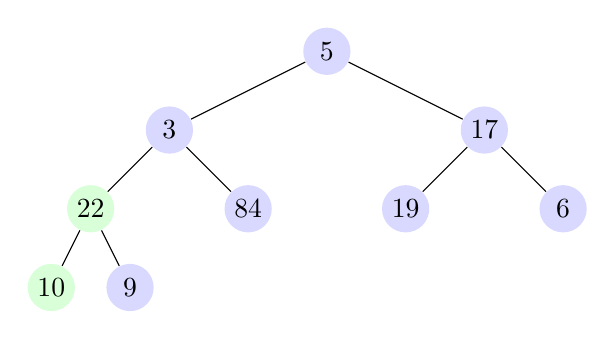
\begin{tikzpicture}
  [level distance = 10mm, node distance=0.1,
   every node/.style={fill=blue!15!white,circle, inner sep=1pt, minimum size=6mm},
   level 1/.style={sibling distance = 40mm},
   level 2/.style={sibling distance = 20mm},
   level 3/.style={sibling distance = 10mm}]
  \node {5}
     child {node{3}
       child {node   [fill=green!15!white,circle]  {22}
          child {node [fill=green!15!white,circle]  {10}}
          child {node {9}}}
       child {node {84}
          child  [missing]
          child [missing]}
     }
     child {node {17}
       child {node {19}
          child  [missing]
          child [missing]}
       child {node {6}
          child  [missing]
          child [missing]}
     };
\end{tikzpicture}
    \captionof{figure}{(b)}
   \label{tikz}
\vspace{30pt}

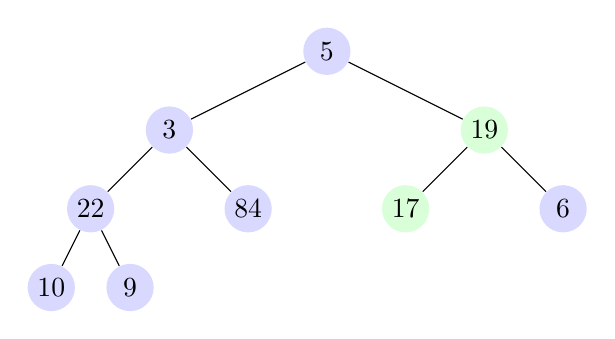
\begin{tikzpicture}
  [level distance = 10mm, node distance=0.1,
   every node/.style={fill=blue!15!white,circle, inner sep=1pt, minimum size=6mm},
   level 1/.style={sibling distance = 40mm},
   level 2/.style={sibling distance = 20mm},
   level 3/.style={sibling distance = 10mm}]
  \node {5}
     child {node{3}
       child {node {22}
          child {node {10}}
          child {node {9}}}
       child {node {84}
          child  [missing]
          child [missing]}
     }
     child {node  [fill=green!15!white,circle] {19}
       child {node[fill=green!15!white,circle] {17}
          child  [missing]
          child [missing]}
       child {node {6}
          child  [missing]
          child [missing]}
     };
\end{tikzpicture}
    \captionof{figure}{(c)}
   \label{tikz}
\vspace{30pt}

\columnbreak
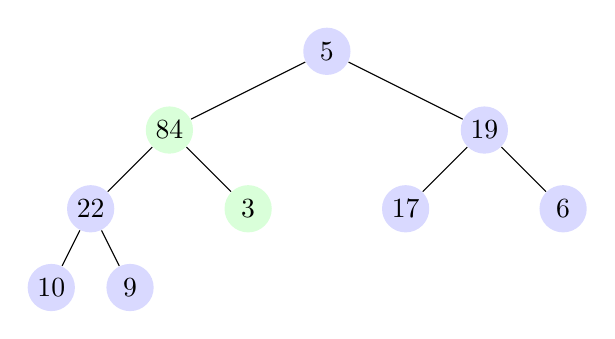
\begin{tikzpicture}
  [level distance = 10mm, node distance=0.1,
   every node/.style={fill=blue!15!white,circle, inner sep=1pt, minimum size=6mm},
   level 1/.style={sibling distance = 40mm},
   level 2/.style={sibling distance = 20mm},
   level 3/.style={sibling distance = 10mm}]
  \node {5}
     child  {node  [fill=green!15!white,circle]  {84}
       child {node {22}
          child {node {10}}
          child {node {9}}}
       child {node [fill=green!15!white,circle] {3}
          child  [missing]
          child [missing]}
     }
     child {node{19}
       child {node {17}
          child  [missing]
          child [missing]}
       child {node {6}
          child  [missing]
          child [missing]}
     };
\end{tikzpicture}
    \captionof{figure}{(d)}
   \label{tikz}
\vspace{30pt}

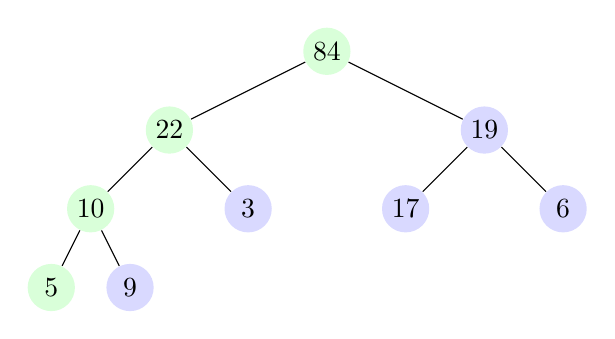
\begin{tikzpicture}
  [level distance = 10mm, node distance=0.1,
   every node/.style={fill=blue!15!white,circle, inner sep=1pt, minimum size=6mm},
   level 1/.style={sibling distance = 40mm},
   level 2/.style={sibling distance = 20mm},
   level 3/.style={sibling distance = 10mm}]
  \node   [fill=green!15!white,circle] {84}
     child  {node [fill=green!15!white,circle] {22}
       child {node [fill=green!15!white,circle] {10}
          child {node [fill=green!15!white,circle] {5}}
          child {node {9}}}
       child {node {3}
          child  [missing]
          child [missing]}
     }
     child {node{19}
       child {node {17}
          child  [missing]
          child [missing]}
       child {node {6}
          child  [missing]
          child [missing]}
     };
\end{tikzpicture}
    \captionof{figure}{(e)}
   \label{tikz}
\vspace{30pt}
\end{center}
\end{multicols}

\newpage
\section*{Exercises 6.4}\nointerlineskip
\noindent \rule{\linewidth}{0.01pt}\\

\subsubsection*{Question 6.4-1}\nointerlineskip
Illustrate \textcolor{blue}{\textbf{HEAPSORT}} on the array $\langle 5,13,2,25,7,17,20,8,4 \rangle$.\\
(Running time: \textcolor{blue}{$\mathcal{O}(n \text{ lg } n)$})\\

\begin{center}
\begin{multicols}{2}
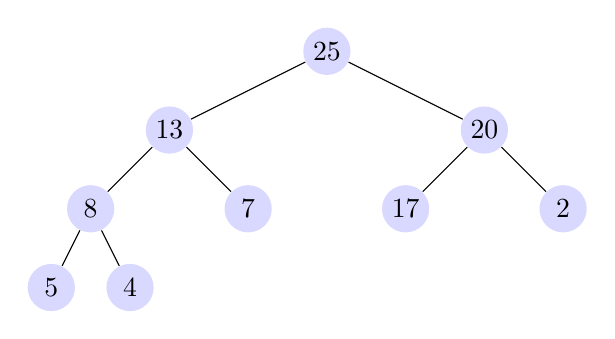
\begin{tikzpicture}
  [level distance = 10mm, node distance=0.1,
   every node/.style={fill=blue!15!white,circle, inner sep=1pt, minimum size=6mm},
   level 1/.style={sibling distance = 40mm},
   level 2/.style={sibling distance = 20mm},
   level 3/.style={sibling distance = 10mm}]
  \node {25}
     child {node{13}
       child {node {8}
          child {node {5}}
          child {node {4}}}
       child {node {7}
          child  [missing]
          child [missing]}
     }
     child {node {20}
       child {node {17}
          child  [missing]
          child [missing]}
       child { node {2}
          child  [missing]
          child [missing]}
     };
\end{tikzpicture}
    \captionof{figure}{(a) After BUILD MAX-HEAP}
   \label{tikz}
\vspace{30pt}

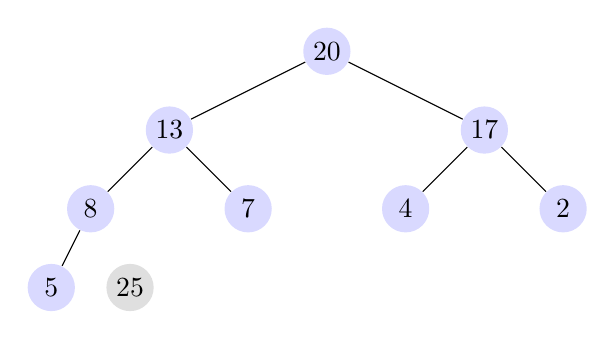
\begin{tikzpicture}
  [level distance = 10mm, node distance=0.1,
   every node/.style={fill=blue!15!white,circle, inner sep=1pt, minimum size=6mm},
   level 1/.style={sibling distance = 40mm},
   level 2/.style={sibling distance = 20mm},
   level 3/.style={sibling distance = 10mm}]
  \node {20}
     child {node{13}
       child {node {8}
          child {node  {5}}
          child [color=white] {node  [fill=gray!25!white,circle][text=black]  {25}}}
       child {node {7}
          child  [missing]
          child [missing]}
     }
     child {node{17}
       child {node {4}
          child  [missing]
          child [missing]}
       child {node {2}
          child  [missing]
          child [missing]}
     };
\end{tikzpicture}
    \captionof{figure}{(b)}
   \label{tikz}
\vspace{30pt}

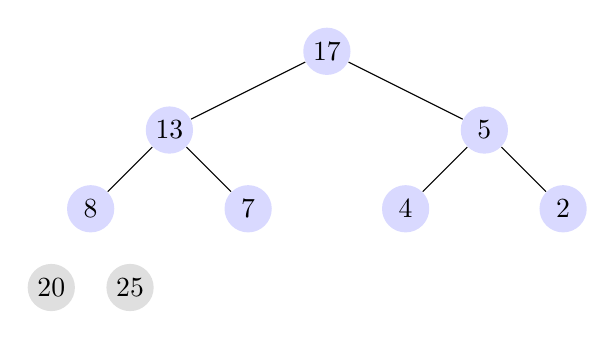
\begin{tikzpicture}
  [level distance = 10mm, node distance=0.1,
   every node/.style={fill=blue!15!white,circle, inner sep=1pt, minimum size=6mm},
   level 1/.style={sibling distance = 40mm},
   level 2/.style={sibling distance = 20mm},
   level 3/.style={sibling distance = 10mm}]
  \node {17}
     child {node{13}
       child {node {8}
          child [color=white]{node [fill=gray!25!white,circle][text=black]   {20}}
          child [color=white] {node [fill=gray!25!white,circle][text=black]  {25}}}
       child {node {7}
          child  [missing]
          child [missing]}
     }
     child {node{5}
       child {node {4}
          child  [missing]
          child [missing]}
       child {node {2}
          child  [missing]
          child [missing]}
     };
\end{tikzpicture}
    \captionof{figure}{(c)}
   \label{tikz}
\vspace{30pt}

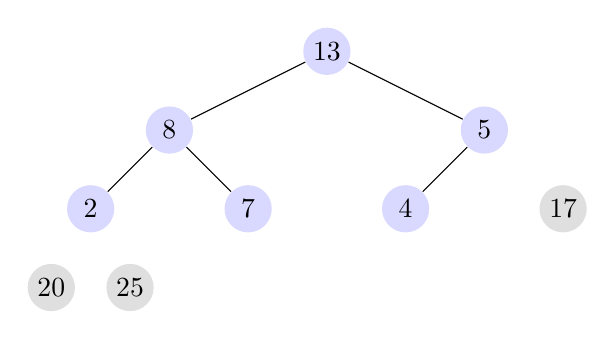
\begin{tikzpicture}
  [level distance = 10mm, node distance=0.1,
   every node/.style={fill=blue!15!white,circle, inner sep=1pt, minimum size=6mm},
   level 1/.style={sibling distance = 40mm},
   level 2/.style={sibling distance = 20mm},
   level 3/.style={sibling distance = 10mm}]
  \node {13}
     child {node{8}
       child {node {2}
          child [color=white]{node [fill=gray!25!white,circle][text=black]   {20}}
          child [color=white] {node [fill=gray!25!white,circle][text=black]  {25}}}
       child {node {7}
          child  [missing]
          child [missing]}
     }
     child {node{5}
       child {node {4}
          child  [missing]
          child [missing]}
       child [color=white]{node[fill=gray!25!white,circle][text=black]{17}
          child  [missing]
          child [missing]}
     };
\end{tikzpicture}
    \captionof{figure}{(d)}
   \label{tikz}
\vspace{30pt}

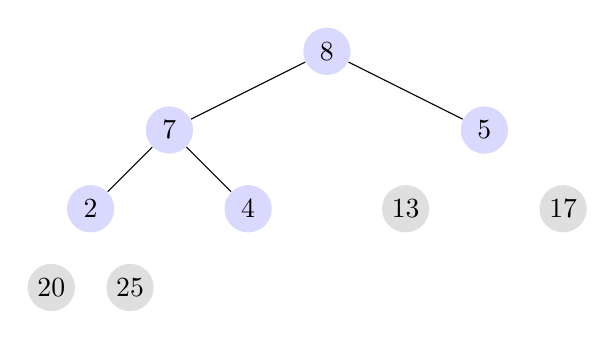
\begin{tikzpicture}
  [level distance = 10mm, node distance=0.1,
   every node/.style={fill=blue!15!white,circle, inner sep=1pt, minimum size=6mm},
   level 1/.style={sibling distance = 40mm},
   level 2/.style={sibling distance = 20mm},
   level 3/.style={sibling distance = 10mm}]
  \node {8}
     child {node{7}
       child {node {2}
          child [color=white]{node [fill=gray!25!white,circle][text=black]   {20}}
          child [color=white] {node [fill=gray!25!white,circle][text=black]  {25}}}
       child {node {4}
          child  [missing]
          child [missing]}
     }
     child {node{5}
       child [color=white] {node [fill=gray!25!white,circle][text=black] {13}
          child  [missing]
          child [missing]}
       child [color=white]{node[fill=gray!25!white,circle][text=black]{17}
          child  [missing]
          child [missing]}
     };
\end{tikzpicture}
    \captionof{figure}{(e)}
   \label{tikz}
\vspace{30pt}

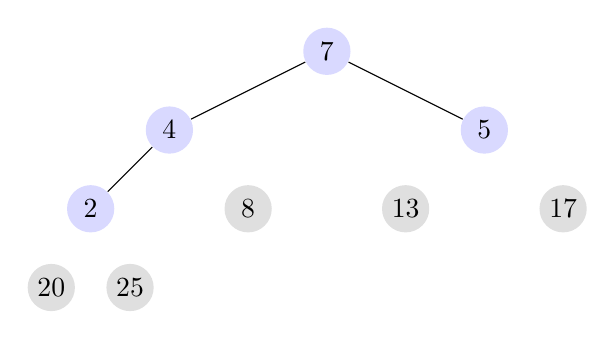
\begin{tikzpicture}
  [level distance = 10mm, node distance=0.1,
   every node/.style={fill=blue!15!white,circle, inner sep=1pt, minimum size=6mm},
   level 1/.style={sibling distance = 40mm},
   level 2/.style={sibling distance = 20mm},
   level 3/.style={sibling distance = 10mm}]
  \node {7}
     child {node{4}
       child {node {2}
          child [color=white]{node [fill=gray!25!white,circle][text=black]   {20}}
          child [color=white] {node [fill=gray!25!white,circle][text=black]  {25}}}
       child  [color=white]{node [fill=gray!25!white,circle][text=black]  {8}
          child  [missing]
          child [missing]}
     }
     child {node{5}
       child [color=white] {node [fill=gray!25!white,circle][text=black] {13}
          child  [missing]
          child [missing]}
       child [color=white]{node[fill=gray!25!white,circle][text=black]{17}
          child  [missing]
          child [missing]}
     };
\end{tikzpicture}
    \captionof{figure}{(f)}
   \label{tikz}
\vspace{30pt}

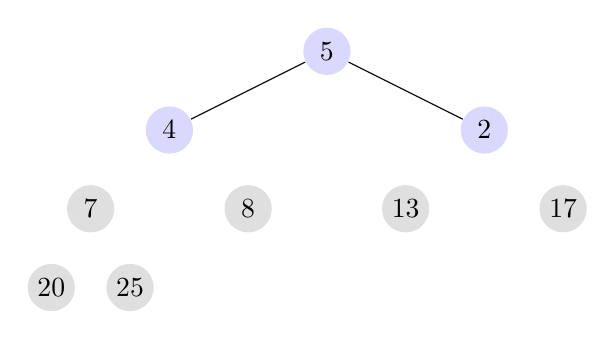
\begin{tikzpicture}
  [level distance = 10mm, node distance=0.1,
   every node/.style={fill=blue!15!white,circle, inner sep=1pt, minimum size=6mm},
   level 1/.style={sibling distance = 40mm},
   level 2/.style={sibling distance = 20mm},
   level 3/.style={sibling distance = 10mm}]
  \node {5}
     child {node{4}
       child [color=white]{node  [fill=gray!25!white,circle][text=black] {7}
          child [color=white]{node [fill=gray!25!white,circle][text=black]   {20}}
          child [color=white] {node [fill=gray!25!white,circle][text=black]  {25}}}
       child  [color=white]{node [fill=gray!25!white,circle][text=black]  {8}
          child  [missing]
          child [missing]}
     }
     child {node{2}
       child [color=white] {node [fill=gray!25!white,circle][text=black] {13}
          child  [missing]
          child [missing]}
       child [color=white]{node[fill=gray!25!white,circle][text=black]{17}
          child  [missing]
          child [missing]}
     };
\end{tikzpicture}
    \captionof{figure}{(g)}
   \label{tikz}
\vspace{30pt}

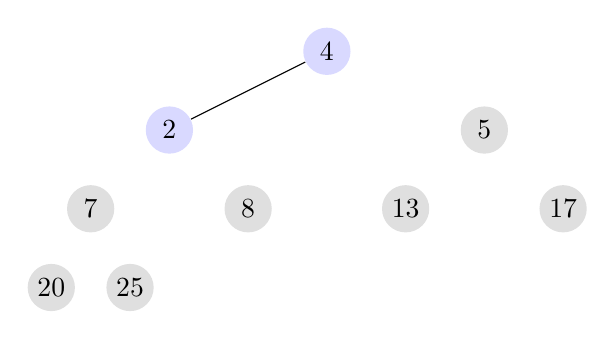
\begin{tikzpicture}
  [level distance = 10mm, node distance=0.1,
   every node/.style={fill=blue!15!white,circle, inner sep=1pt, minimum size=6mm},
   level 1/.style={sibling distance = 40mm},
   level 2/.style={sibling distance = 20mm},
   level 3/.style={sibling distance = 10mm}]
  \node {4}
     child {node{2}
       child [color=white]{node  [fill=gray!25!white,circle][text=black] {7}
          child [color=white]{node [fill=gray!25!white,circle][text=black]   {20}}
          child [color=white] {node [fill=gray!25!white,circle][text=black]  {25}}}
       child  [color=white]{node [fill=gray!25!white,circle][text=black]  {8}
          child  [missing]
          child [missing]}
     }
     child [color=white]{node [fill=gray!25!white,circle][text=black] {5}
       child [color=white] {node [fill=gray!25!white,circle][text=black] {13}
          child  [missing]
          child [missing]}
       child [color=white]{node[fill=gray!25!white,circle][text=black]{17}
          child  [missing]
          child [missing]}
     };
\end{tikzpicture}
    \captionof{figure}{(h)}
   \label{tikz}
\vspace{30pt}
\columnbreak

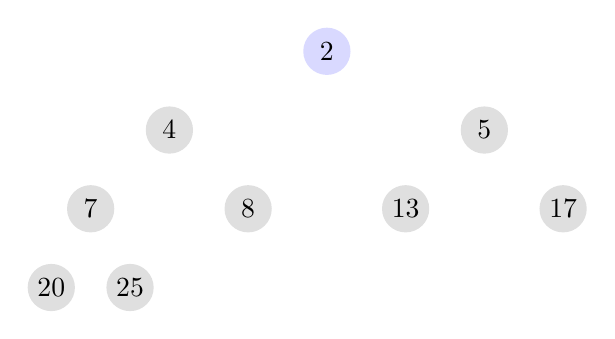
\begin{tikzpicture}
  [level distance = 10mm, node distance=0.1,
   every node/.style={fill=blue!15!white,circle, inner sep=1pt, minimum size=6mm},
   level 1/.style={sibling distance = 40mm},
   level 2/.style={sibling distance = 20mm},
   level 3/.style={sibling distance = 10mm}]
  \node {2}
     child [color=white]{node [fill=gray!25!white,circle][text=black] {4}
       child [color=white]{node  [fill=gray!25!white,circle][text=black] {7}
          child [color=white]{node [fill=gray!25!white,circle][text=black]   {20}}
          child [color=white] {node [fill=gray!25!white,circle][text=black]  {25}}}
       child  [color=white]{node [fill=gray!25!white,circle][text=black]  {8}
          child  [missing]
          child [missing]}
     }
     child [color=white]{node [fill=gray!25!white,circle][text=black] {5}
       child [color=white] {node [fill=gray!25!white,circle][text=black] {13}
          child  [missing]
          child [missing]}
       child [color=white]{node[fill=gray!25!white,circle][text=black]{17}
          child  [missing]
          child [missing]}
     };
\end{tikzpicture}
    \captionof{figure}{(i)}    
\vspace{120pt}

\begin{tabular}{ |c|c|c|c|c|c|c|c|c| } 
 \hline
 2 & 4 & 5 & 7 & 8 & 13  & 17 & 20 & 25 \\ 
 \hline
\end{tabular}
    \captionof{figure}{(j)}
\end{multicols}
\end{center}


\vspace{20pt}

\subsubsection*{Question 6.4-3}\nointerlineskip
What is the running time of HEAPSORT on an array $A$ of length $n$ that is already sorted in increasing order? What about decreasing order?\\

Even though it's sorted, the first line of HEAPSORT calls BUILD-MAX-HEAP and we know the running time for that is $\mathcal{O}(n)$. It then calls MAX-HEAPIFY for all the nodes, and the running time for MAX-HEAPIFY is $\mathcal{O}($lg $n)$. So the total running time for Heapsort, regardless of the order of the array, is $\mathcal{O}(n$ lg $n)$. \\

\end{document}